\chapter{Range min-Max tree k-ária}
\label{chp:desenvolvimento}
Esta capítulo refere-se ao objetivo central deste trabalho, apresentando a proposta de otimização da estrutura criada por \cite{paper-fully-functinal-succint-trees}.
Mostraremos primeiro no que consiste essa adaptação, após isso definiremos a forma como serão compostos os nós da rmM-tree e como a mesma deve ser construída,
apresentaremos também as operações suportadas por esta estrutura, detalhando as princpipais delas. 
Por fim, destaca-se que os exemplos usados como base neste capítulo, 
serão os mesmos exemplos usado no capítulo de apresentação da rmM-tree clássica, afim de facilitar a compreensão e comparação das duas propostas.

\section{Visão Geral}
Para este trabalho buscamos unir algumas características das árvores B com a range min-Max tree. 
Com até $m$ filhos, as árvores B possuem altura igual a $\log_m n$ e alto fator de ramificação, essas características combinadas a Range min-Max tree,
que é uma estrutura compacta, e portanto cabe na memória principal, possibilitará um uso otimizado de cache. Pois o alto fator de ramificação da estrutura,
implicará em um uso satisfatório do príncipio de localidade de dados, e em decorrência disto em uma diminuição do número de cache misses 
\citep{paper-making-btree-cache}.

Ademais, como também mostram \citet{paper-effect-node-size-cache-b-trees} o número de faltas de cache é limitado pela altura da árvore,
o que como já expomos é menor para as árvores B, espera-se assim reduzir o tempo para as operações sobre a rmM-tree k-ária, se comparada ao
tempo gasto pelas operações na rmM-tree binária.
Por último, vale ressaltar que a complexidade assintótica das duas estruturas será a mesma, 
porém devido ao número reduzido de transferência de dados entre cache e memória RAM, 
a constante oculta desse limite assintótico será reduzida \citep{book-algoritmos-teoria-pratica}, melhorando o desempenho do sistema.

Assim, dado uma representação compacta de uma árvore geral $T$, na forma de parênteses balanceados, ou vetores de bits, 
é escolhido um tamanho de bloco $b$, esse tamanho de bloco, assim como na estrutura clássica define a cobertura de um determinado 
intervalo. 
Na proposta original \citep{paper-fully-functinal-succint-trees}, cada nó da Range min-Max tree é responsável pela cobertura de um desses intervalos. 
Nesta adaptação propõe-se o agrupamento múltiplo de intervalos no formato de chaves em nós.

Com base nisso, após definir uma ordem $m$, com $m$ maior que 2, para a rmM-tree, armazenaremos $m$ chaves  \footnote{Uma árvore B armazena até m-1 chaves por página, aqui optamos por manter $m$ chave,
por nó, afim de garantir uma cobertura completa dos intervalos à cada nível},
contendo intervalos de máximos e mínimos  de tamanho $b$ por nó da nossa estrutura.
Isso implica que teremos até  $m^2$  áreas cobertas por nó  (pois $m \mbox{ filhos } \cdot (m) $ chaves), dessa maneira temos o exposto:
se na versão clássica  da rmM-tree cada nó folha armazena no máximo um intervalo, e portanto possuí $r=\ceil{n/b}$ folhas, 
na versão k-ária teremos $r=\ceil{n/(b \cdot m)}$ folhas.

Como a altura de uma árvore pode ser calculada a partir de $h = \ceil{\log_m r}$ essa simples mudança reduzirá drasticamente a altura da nossa estrutura,
quando comparada a rmM-tree clássica,  fazendo com que o número de eventuais transferências de dados entre os níveis da memória torne-se menor.

Tomemos como exemplo um tamanho de bloco $b = 32$, suponha um vetor de bits de tamanho igual à  $4.675.776.358$, e que a nossa rmM-tree tem ordem $16$, o exemplo logo abaixo
ajuda a esclarecer o expostos acima, mostrando a altura, quantidade de folhas de cada versão da rmM-tree.

\begin{eqnarray*}
    r = \ceil{4.675.776.358/32} = 146.118.012 \\
    h = \ceil{\log_2(146.118.012)} = 28  \mbox{, para a estrutura clássica}.\\
    \\
    r = \ceil{(4.675.776.358/(32 \cdot 16))} = 9.132.376 \\
    h = \ceil{\log_{16}(4.711.244)} = 6  \mbox{, para a estrutura otimizada}.
\end{eqnarray*}

No pior caso do exemplo acima, a rmM-tree clássica terá 28 transferências de dados entre os níveis da hierarquia de memória, ao passo que no pior caso da rmM-tree otimizada teremos 6 
transferências. Isso acontece porque ao aumentar o número de dados cobertos por nós, tiramos proveito do príncipio de localidade espacial \citep{book-computer-architecutre}.
Assim a estrutura da nossa árvore ao maximizar o volume de dados enviados a cada transferência, faz com que os mesmo sejam referenciados de modo mais rápido.
%pg 524
\section{Registros}
Os registros da range min-Max tree k-ária permanecem exatamente os mesmos, sendo eles: \textit{excesso local (e)}, que indica o excesso total 
computado em um intervalo; \textit{excesso local mínimo (m)} que é relativo ao menor exesso computado a cada posição do intervalo $[s,e]$;
 \textit{excesso local máximo (M)} que é análogo ao excesso mínimo; e \textit{número de vezes que o excesso mínimo ocorre (n)} em um intervalo. 
 A grande diferença, é que agora esses valores de excessos estão agrupados em até $m$ blocos de tamanho $b$ por folha, isso nos dá às seguintes relações
 para os nós internos e raíz:

\begin{itemize}
    \item $R[v][k].e = \displaystyle{\sum_{i=0}^{l-1} R[j][i].e} $
    \item $R[v][k].m = min(R[j][0].m, ... , R[j][0].e + ... + R[j][l-1].e + R[j][l].m )$
    \item $R[v][k].M = Max(R[j][0].M, ... , R[j][0].e + ... + R[j][l-1].e + R[j][l].M )$
    \item $R[v][k].n$ o valor desse registro irá depender da quantidade de vezes que o excesso mínimo computado aparece entre as chaves do nó $j$.
    Caso esse valor não se repita, o valor de $n$, em $v$, será definido pelo valor de $n$ na chave que contém o excesso mínimo,
    caso contrário, $R[v][k].n$ será dado pelo somatório de $n$, nas chaves do nó $j$ onde o excesso mínimo se repete. 
\end{itemize}

onde:
\begin{itemize}
    \item $k$, é a $k-$ésima chave de $v$ e aponta para o nó $(v*m)+1+k$ (com $0 \leq k <  m$ );
    \item $j$ é o $j-$ésimo filho de $v$;
    \item $l$ é a quantidade de chaves em $j$.
\end{itemize}


\begin{example}
%TODO
Usando o mesmo exemplo de sequência de parênteses balanceados da seção~\ref{sec:sec-classic-rmm-tree},
assuma a cobertura de bloco igual à $4$, e uama rmM-tree de  ordem também igual à $4$. 
Temos assim que a Range min-Max tree terá 4 nós folhas, e no máximo $4$ chaves por nó, pois:

$$r = \ceil{n/(b \cdot m)} \to \ceil{(52/16)} = 4$$
$$h = \ceil{\log_m r} \to \ceil{\log_4 4} = 1 $$

%Na fundamentação
Como nesta adaptação as chaves da rmM-tree assumem o papel dos blocos da implementação clássica, as chaves dos nós folhas serão idênticas às folhas
definidas no exemplo~\ref{ex-build-tree}, em ordem. 
Iremos portanto nos concentrar em exemplificar a forma como é feito o cálculo de 1 das chaves
de um dos nós superiores da nossa estrutura, que devido às características da nossa árvore base, será o nó raíz:


Tomemos a chave de número 2, do nó raíz da nossa estrutura, o nó ao qual está chave se refere, é o nó $v = (4*0)+1+2 \therefore v =3$, ou seja, 
temos que os valores para as chaves deste nósão:

\begin{itemize}
    \item Chave 0:\\
    Cobertura: $BP[32,35], e=0, M=1, m=0,n=2$
    \item Chave 1:\\
    Cobertura: $BP[36,39], e=0, M=1, m=-1,n=1$
    \item Chave 2:\\
    Cobertura: $BP[40,43], e=0, M=1, m=0,n=2$
    \item Chave 3:\\
    Cobertura: $BP[43,47], e=0, M=1, m=0,n=2$
\end{itemize}

Assim, a chave $2$, da página raíz, da qual descende está folha terá os seguintes valores:
\begin{itemize}
    \item $R[0].keys[2].e = R[3].keys[0].e + R[3].keys[1].e + R[3].keys[2].e + R[3].keys[3].e=0$
    \item $R[0].keys[2].M = 1$, pois:
    \begin{eqnarray*}
        \begin{split}
            R[0].keys[2].M =& max(R[3].keys[0].M, \\
            &   R[3].keys[0].e + R[3].keys[1].M, \\
            &  R[3].keys[0].e + R[3].keys[1]. e + R[3].keys[2].M,  \\
            &   R[3].keys[0].e + R[3].keys[1]. e + R[3].keys[2].e +  R[3].keys[3].M)\\
            &  max(1, 1, 1,1) = 1
        \end{split}
    \end{eqnarray*}
        
    \item $R[0].keys[2].m = -1$, pois:
    \begin{eqnarray*}
        \begin{split}
            R[0].keys[2].M =& min(R[3].keys[0].m, \\
            &   R[3].keys[0].e + R[3].keys[1].m, \\
            &  R[3].keys[0].e + R[3].keys[1]. e + R[3].keys[2].m,  \\
            &   R[3].keys[0].e + R[3].keys[1]. e + R[3].keys[2].e +  R[3].keys[3].m)\\
            &   min(0,-1,0,0) = -1
        \end{split}
    \end{eqnarray*}
    
    \item $R[0].keys[2].n = 1$, pois o excesso ocorre uma única vez, na chave de número $1$ do nó $3$ (folha $2$).
\end{itemize}

Tendo computado os valores de excesso máximo e mínimo para todas as chaves dos nós folhas, e posteriormente para a raíz, temos a rmM-tree da \figref{fig:rmm-tree-k}:
    \begin{figure}[h!]
    \centering
      \caption[rmM-tree 4-ária.]{rmM-tree 4-ária, com tamanho de bloco igual à 4. No canto superior esquerdo de cada nó, em negrito,
        é mostrado o índice do mesmo na rmM-tree, já no canto inferior esquerdo de cada folha, em azul, vemos a ordem da mesma.}
      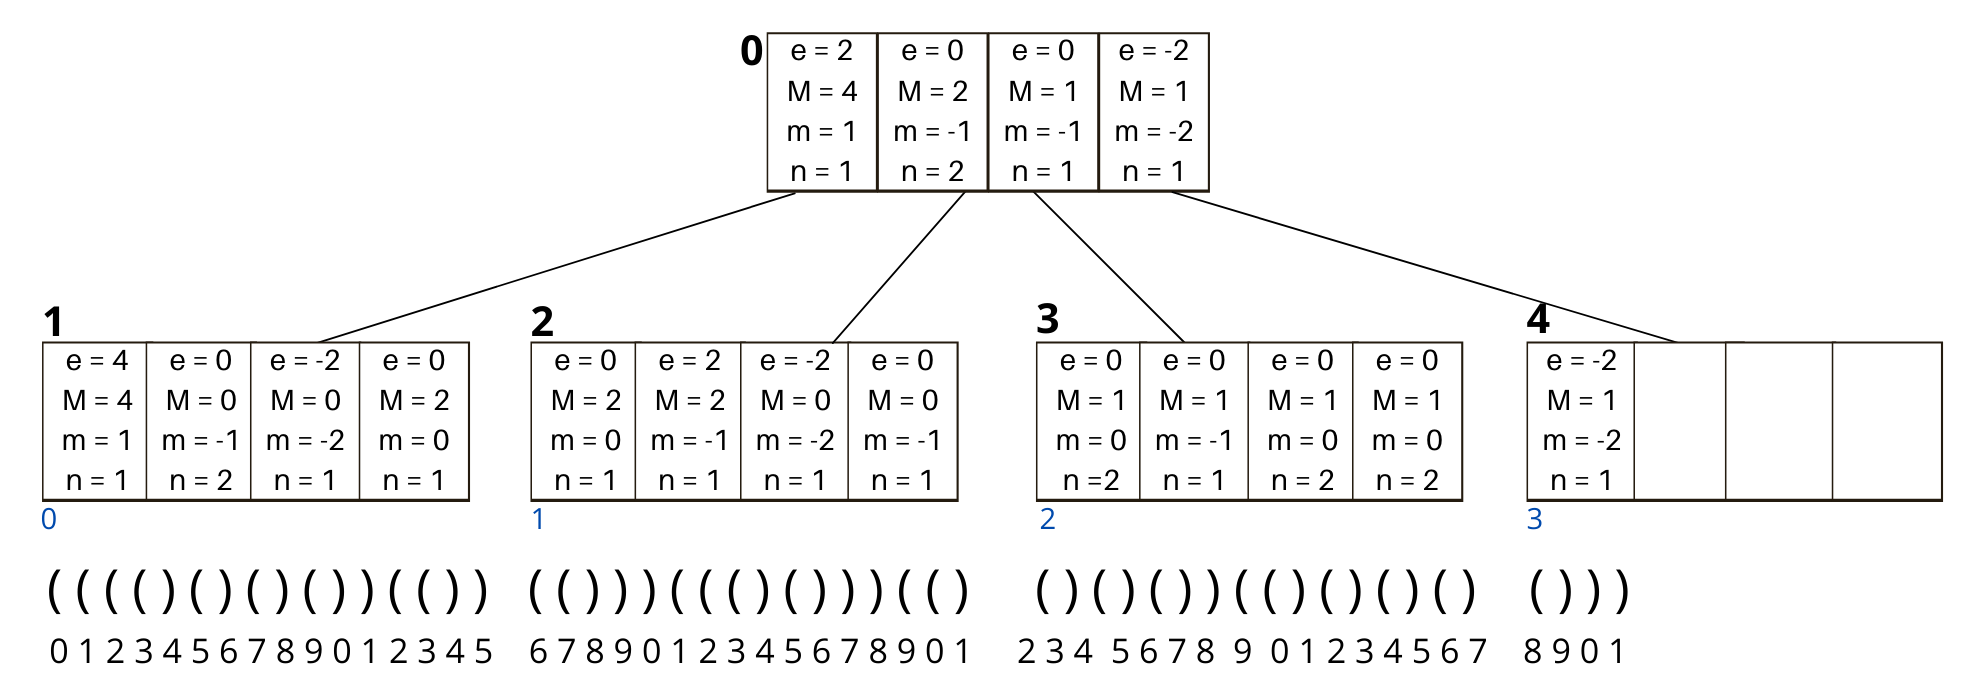
\includegraphics[width=\columnwidth]{images/rmm-tree-kary.png}
      \label{fig:rmm-tree-k}
    \end{figure}
    
\end{example}

O processo de construção da rmM-tree k-ária é similar ao processo de construção da rmM-tree binária descrito no capítulo~\ref*{ch:fundamentacao},
 a diferença é que, para este caso precisaremos guardar em um nó até $m$ registros de excesso. Podemos para tanto fazer o uso de uma estrutura auxiliar como
 uma lista ou um vetor (presente em linguagens de programação como C++), onde cada elemento dessa estrutura representará as chaves, de um nó $v$ da rmM-tree, ao qual essa estrutura auxiliar está
 associada.
 Veja como isso pode ser feito usando o algoritmo \ref{alg:build-kary-rmm-tree}. A tabela C, as funções \textit{bitsread, leafInTree} e 
 \textit{numLeaf}, algumas citadas nesse e outras em outros algoritmos seguem a mesma abordagem da rmM-tree clássica. 
\begin{algorithm}[h!]
    \Input{$BP[0,n-1]$, tabela C, tamanho de bloco $b$ e de sub-bloco $w$ (com $b$ mod $w = 0$), número de folhas $r$, quantidade de nós $nNodes$ }

    \tcp{Construção dos nós folhas}
    $numKey \leftarrow 0$\\
    \For{$k \leftarrow 0$ \textbf{to} $r -1$}{
        $v \leftarrow leafInTree(k); key \leftarrow 0$\\
        \While{$R[v].nKeys < m$ \textbf{and} $nunKey \leq \ceil{BP.size()/b}$}{
            $R[v].keys[key].e \leftarrow 0; R[v].keys[key].m \leftarrow -w;$\\ 
            $R[v].keys[key].M \leftarrow w; R[v].keys[key].n \leftarrow 0;$\\
            \For{$p \leftarrow (numKey*(b/w))+1$ \textbf{to} $((numKey+1)*b)/w$}{
                $x \leftarrow bistread((p-1)*w)$\\
                \lIf{$R[v].keys[key].e + C[x].M > R[v].keys[key].M$}{$R[v].keys[key].M \leftarrow R[v].keys[key].e + C[x].M $}
                \lIf{$R[v].keys[key].e + C[x].m < R[v].keys[key].m$}{$R[v].keys[key].m \leftarrow R[v].keys[key].e + C[x].m $}
                \ElseIf{$R[v].keys[key].e + C[x].m = R[v].keys[key].m$}{$R[v].keys[key].n \leftarrow R[v].keys[key].n + C[x].n$}
                $R[v].keys[key].e \leftarrow R[v].keys[key].e + C[x].e$
            }
            $R[v].nKeys \leftarrow R[v].nKeys  +1$\\
            $numKey \leftarrow numKey +1$\\
            $key \leftarrow key +1$

        } 
    }
    \tcp{Construção dos nós internos e raíz}
    \For{$v \leftarrow nNodes - r - 1 $ \textbf{to} $0$}{
        \For{$key \leftarrow 0$ \textbf{to} $m-1$ \textbf{and} $(v*m)+key+1$ \textbf{to} $nNodes-1$}{
            $child \leftarrow (m*v)+1+key$\\
            $R[v].keys[key].e \leftarrow R[child].keys[0].e$\\
            $R[v].keys[child].m \leftarrow R[child].keys[0].m$\\
            $ R[v].keys[child].M \leftarrow R[child].keys[0].M$\\
            $R[v].keys[child].n \leftarrow R[child].keys[0].n$\\
            \For{$i \leftarrow 1$ \textbf{to} $R[child].nKeys-1$}{
                $R[v].keys[key].M = max(R[child].keys[i].M,R[v].keys[i-1].e + R[child].keys[i].M) $\\
                $R[v].keys[key].m = max(R[child].keys[i].m,R[v].keys[i-1].e + R[child].keys[i].m) $\\
                \If{$R[child].keys[i].m < R[v].keys[i-1].e + R[child].keys[i].m$}{
                    $R[v].keys[key].n \leftarrow R[child].keys[i].n$
                }
                \lElseIf{$R[child].keys[i].m = R[v].keys[i-1].e + R[child].keys[i].m$}{
                    $R[v].keys[key].n \leftarrow R[child].keys[i].n + R[child].keys[i-1].n$
                }
                $R[v].keys[key].e \leftarrow R[child].keys[i].e$\\
            }
        }

    }
    \caption{Construção da range min-Max tree k-ária}
    \label{alg:build-kary-rmm-tree}
\end{algorithm} 

\section{Operações}\label{sec:optimized-operation}
Para este trabalho a nossa estrutura fornece suporte às duas principais primitivas da Range min-Max tree clássica,
FwdSearch e BwdSearch (além daquelas já suportadas pela estrutura de vetores de bits).
Além destas duas, nossa árvore de intervalos máximos e mínimos, fornece suporte à 5 operações derivadas daquelas apoiadas pela estrutura de vetores
de bits (sobre a qual a nossa árvore é construída), e outras 16 operações, que são derivadas das duas primitivas exploradas adiante.


\subsection{FwdSearch}\label{sec:fwdSearch}
Como já dito no capítulo anterior a operação foward search, realiza uma busca a partir de um índice \textit{i}, afim de encontrar a posição $j$, onde ocorre um excesso relativo \textit{d}.

Essa operação, nessa versão da rmM-tree, se dá parcialmente de igual forma ao do modo clássico, varremos primeiro o bloco da folha,
de \textit{w} em \textit{w} bits em busca do excesso desejado, a partir de $i+1$. 
A diferença é que agora precisamos verificar por até \textit{m} blocos de tamanho \textit{b} dentro dos nós da nossa estrutura.
Para tanto, acrescentamos à fwdSearch em sua versão clássica duas outras funções, são elas fwdKey e fwdVerifySibling.

A primeira função é chamada sempre que estamos visitando um nó folha, ou seja no ínicio da busca e ao final da mesma, quando já encontramos o nó alvo que contém a resposta. 
FwdKey tem por objetivo verificar as chaves do nó visitado, em busca daquela cujo os campos de intervalo máximo e mínimo compreendem o excesso relativo \textit{d}.
O processo é muito similar à verificação de um nó, a cada chave pecorrida verificamos se a asserção $dr + R[v].key[l].m \leq d \leq dr + R[v].key[l].M$, caso a asserção seja 
significa que encontramos o intervalo que contém a resposta desejada, então nos encaminhamos para a função fwdBlock algoritmo~\ref{alg:fwdBlock}, que fará uma varredura bit-a-bit da chave que contém a resposta.
Se a asserção acima for falsa, adicionamos a \textit{dr} o excesso local da chave que acabamos de visitar, e prosseguimos para a próxima chave. 
O algoritmo \ref{alg:fwdKey} fornece mais detalhes de como esse processo de busca por excesso nas folhas funciona.

\begin{algorithm}[h!]
    \Input{Nó $v$, e folha correspondente $k$, posição a partir do qual devemos iniciar a busca (índice $i$ e $key$),  excesso
    relativo buscado, e excesso relativo computado em cada chave inspecionada ($d$ e $\&dr$). }
    \Output{Posição $j$ ou $BP.size()$ caso $d$ não seja encontrado.}
    \vspace{.3cm}
        \For{$key$ \textbf{to}  $R[v].nKeys -1$}{
            \If{$(dr + R[v].keys[key].m  \leq  d \leq  dr + R[v].keys[key].M)$}{
                $j \leftarrow fwdBlock(i,d,dr)$\tcp{Algoritmo~\ref{alg:fwdBlock}}
                \If{$dr = d$}{ \Return{$j$ }}

            }
            $dr \leftarrow dr +  R[v].keys[key].e$\\ 
            $i \leftarrow (m*k+key+1)*b -1$ \tcp{calcula o fim da chave atual}
            \If{$dr = d$}{\Return{$i$ }}
        }
        \Return{$BP.size()$}
    \caption{Verificando as chaves de um nó folha através de $fwdKey(i,v,key,k,d,\&dr)$}
    \label{alg:fwdKey}
    \end{algorithm}
    

Caso o excesso \textit{d} não seja encontrado na folha, acionamos o processo de subida na árvore, aliado à nova função que mencionamos, \textit{fwdVerifySibling}.
O objetivo dessa função é similar ao proposto por \citet{book-compact-data-structures}, quando o autor sugere que em cada nível verifiquemos se o excesso procurado está no irmão do nó atual.
Assim \textit{fwdVerifySibling} calcula a quantidade de irmãos do nó $v$ existentes à sua direita - calcula-se o índice do primeiro filho do pai de $v$, e subtraímos de $v$ o resultado, o número de irmãos 
à direita de $v$ é o número chaves do seu pai, subtraído desse resultado - e então 
pecorremos as chaves de cada irmão à direita de $v$, em busca do excesso relativo $d$. O processo de verificação de chaves é similar ao descrito anteriormente, com a diferença de que
se em algum momento dessa varredura encontrarmos o intervalo que contém o excesso relativo desejado, atualizamos $v$ (se $v$ não for um nó folha) para o filho correspondente
à chave que contém a resposta, e interropemos o processo de verificação dos nós irmãos, retornando à \textit{fwdSearch} a chave que contém a resposta, com o nó $v$
atualizado. Tendo achado a resposta, o processo de subida na árvore é interrompido, caso contrário $v$ é atualizado para o índice do seu nó pai e o processo de verificação dos nós irmãos
é repetido.

Após encontrarmos o nó $v$, que contém o excesso  $d$, iniciamos  um estreitamento do intervalo a ser inspecionado, através do processo de descida na
rmM-tree. Esta etapa é muita similar as demais, pecorremos as chaves de $v$ verificando se a asserção $dr + R[v].key[l].m \leq d \leq dr + R[v].key[l].M$ é válida,
atualizando o valor de $dr$, sempre que $d$ não estiver compreendido dentro do intervalo de uma das chaves de $v$, quando a asserção for válida, atualizamos o valor de $v$,
para sua respectiva chave. Repetimos esse processo até que cheguemos à um nó folha, que é quando executamos novamente \textit{fwdKey}, varrendo o nó folha desde a sua primeira chave.
Os algoritmos \ref{alg:fwdVerifySibling} e \ref{alg:fwdSearch} mostram como o processo de descida na árvore funcionam, bem como o funcionamento completo de \textit{fwdSearch}.

    \begin{algorithm}[h!]
        \Input{Nó $\&v$,  excesso relativo buscado e excesso relativo computado em cada chave inspecionada ($d$ e $\&dr$). }
        \Output{$key$ ou $BP.size()$ caso o intervalo que contém $d$ não seja encontrado.}
        \vspace{.3cm}
        $parent \leftarrow \floor{(v-1)/m}$ \\
        $n\_sibling \leftarrow v - (parent * m)$\\
        $v \leftarrow v + 1$\\
        \While{$n\_sibling$ \textbf{to}  $R[parent].nKeys -1$ \textbf{and} $v$ \textbf{to} $num\_nodes - 1$}{
            \For{$key \leftarrow 0$ \textbf{to} $R[v].nKeys -1$}{
                \If{($dr + R[v].keys[key].m  \leq  d \leq  dr + R[v].keys[key].M)$}{
                    \lIf{$v \leq numberNodes - numberLeaves$}{$v \leftarrow (v*m)+1+key$}
                    \Return{$key$ }
                }
                $dr \leftarrow dr +  R[v].keys[key].e$\\
                \If{$dr = d$}{
                    \lIf{$v \leq numberNodes - numberLeaves$}{$v \leftarrow (v*m)+key+2$}
                    \Return{$key+1$ }
                }
            }
            $n\_sibling \leftarrow n\_sibling + 1$\\
            $v \leftarrow v+1$\\
            %TODO preciso ser tão precisa?exibir todas as condições do meu código?Lembrando que estou trabalhando com referencia 
        }
        \Return{$BP.size()$ }
        \caption{Busca o excesso relativo nos irmãos de $v$ através de $fwdVerifySibling(\&v,\&dr,d)$}
        \label{alg:fwdVerifySibling}
    \end{algorithm}

    
    \begin{algorithm}[h!]
        \Input{Índice $i$ a partir do qual a busca deve ser feita e excesso relativo buscado $d$. }
        \Output{Posição $j$ onde ocorre o excesso $d$ ou $BP.size()$ caso $d$ não exista no intervalo definido.}
        \vspace{.3cm}
            $dr \leftarrow 0$\\
            $k \leftarrow \floor{(i+1)/(b*m)}$\\
            $v \leftarrow leafInTree(k)$\\
            $key \leftarrow \floor{( (i+1) - (k*b*m))/b}$\\
            $j \leftarrow fwdBlock(i,d,dr)$\tcp{Algoritmo~\ref{alg:fwdBlock}}

            \lIf{$dr = d $}{\Return{$j$}}

            $key \leftarrow key +1$\\
            \If{$key < R[v].nKeys$}{
                $j \leftarrow fwdKey((m*k+key)*b-1,v,key,k,d,dr)$\\
                \lIf{$dr = d $}{\Return{$j$}}
            }
            \vspace{.3cm}
           \tcp{Inicia o processo de subida na rmM-tree}
            \While{$v \neq 0$ \textbf{and} $fwdVerifySibling(v,dr,d) = BP.size()$ }{
                $v \leftarrow \floor{(v-1)/m}$\\
            }
            
            \tcp{Chegamos ao nó raíz, e $d$ não está em nenhum dos seus filhos}
            \lIf{$v=0$ \textbf{and} $key=v.size()$}{\Return{$v.size()$}}
            \vspace{.3cm}
            \tcp{Inicia descida em árvore}
            \While{$v \leq numberNodes - numberLeaves$}{
                \For{$ke \leftarrow 0$ \textbf{to} $v.nKeys -1$}{
                    \If{$(dr + v[chave].m  \leq  d \leq  dr + v[chave].M)$}{
                        $v \leftarrow (v*m) + 1 + chave $\\
                        $key \leftarrow 0 $\\
                        \textbf{break}
                    }
                    \lElse{
                        $dr \leftarrow dr +  v[chave].e$
                    }

                }
            }
            $k \leftarrow numLeaf(v)$\\
            $i \leftarrow (m*k*chave)*sizeBlock$  \tcp{Calcula o índice inicial da folha que queremos inspecionar}
            $j \leftarrow fwdKey(i-1,v,0,k,d,dr)$\\
            \lIf{$dr = d$}{ \Return{$j$}}
            \Return{$BP.size()$}
        \caption{Busca por excesso no intervalo $[i+1,BP.size()-1]$ através de $fwdSearch(i,d)$}
        \label{alg:fwdSearch}
        \end{algorithm}

        \begin{example}
        Dado um nó em $BP$, codificado em $i=21$, encontrar o primeiro índice $j>i$, tal que $excess(j) - excess(i) = -1$.
   

        O processo para a obtenção dessa resposta é descrito a seguir:
    

         O primeiro passo é identificar  o índice do nó folha que cobre $i=21+1$ (lembrando que a busca é por um $j > i$), neste caso $v = 3$.
         Precisamos também identificar a que chave de $v$, $i$ pertence, temos que $\floor{(21 - 16)/4} = 1$. 
         Iniciamos então a varredura, pecorrendo o nó $v$, a partir de $i+1$ até o final da chave $1$, ao chegar ao final da chave, 
         temos como excesso computado até o momento ($dr$) $2$, e portanto não encontramos o excesso buscado ($d=-1$).

         Como ainda existem chaves em $v$ que não foram inspecionados, pecorremos as chaves restantes, verificando a cada momento se $dr + R[3].keys[l].m \leq d \leq dr + R[3].keys[l].M$
         é válida, passamos pela chave $2$ e não encontramos o excesso buscado, atualizamos o valor de $dr$ somando à ele $R[3].keys[2].e$,
         e inspecionamos a chave $3$,  onde o excesso $dr=d$ finalmente é alcançado.
         Interrompemos a análise dos nós da rmM-tree, e iniciamos uma análise mais detalhada, bit-a-bit da chave $3$, a fim de encontrar a posição exata onde $d$ ocorre.
         Durante essa inspeção, atualizamos o valor de $dr$ em $1$ ao inspecionarmos um bit $1$, e em $-1$ ao visitarmos um bit $0$.
         A varredura bit-a-bit, acontece a partir do ínicio da chave $3$, e já no primeiro índice desta chave temos que $dr=d$, nesse momento significa que encontramos
         a resposta buscada, sendo que ela $j = 28$.


         Perceba que aqui foi necessário a inspeção de $2$ nós (excluindo o nó inicial), sem a necessida de subir na rmM-tree, ao passo que para o mesmo exemplo, na estrutura binária é necessário a inspeção de 
         $5$ nós (excluindo o nó inicial), subir um nível, e depois descer um nível.
         
         \begin{figure}[!ht]
            \centering
              \caption[fwdSearch(21,-1).]{Simulação da operação \textit{fwdSearch(21,-1)}.}
              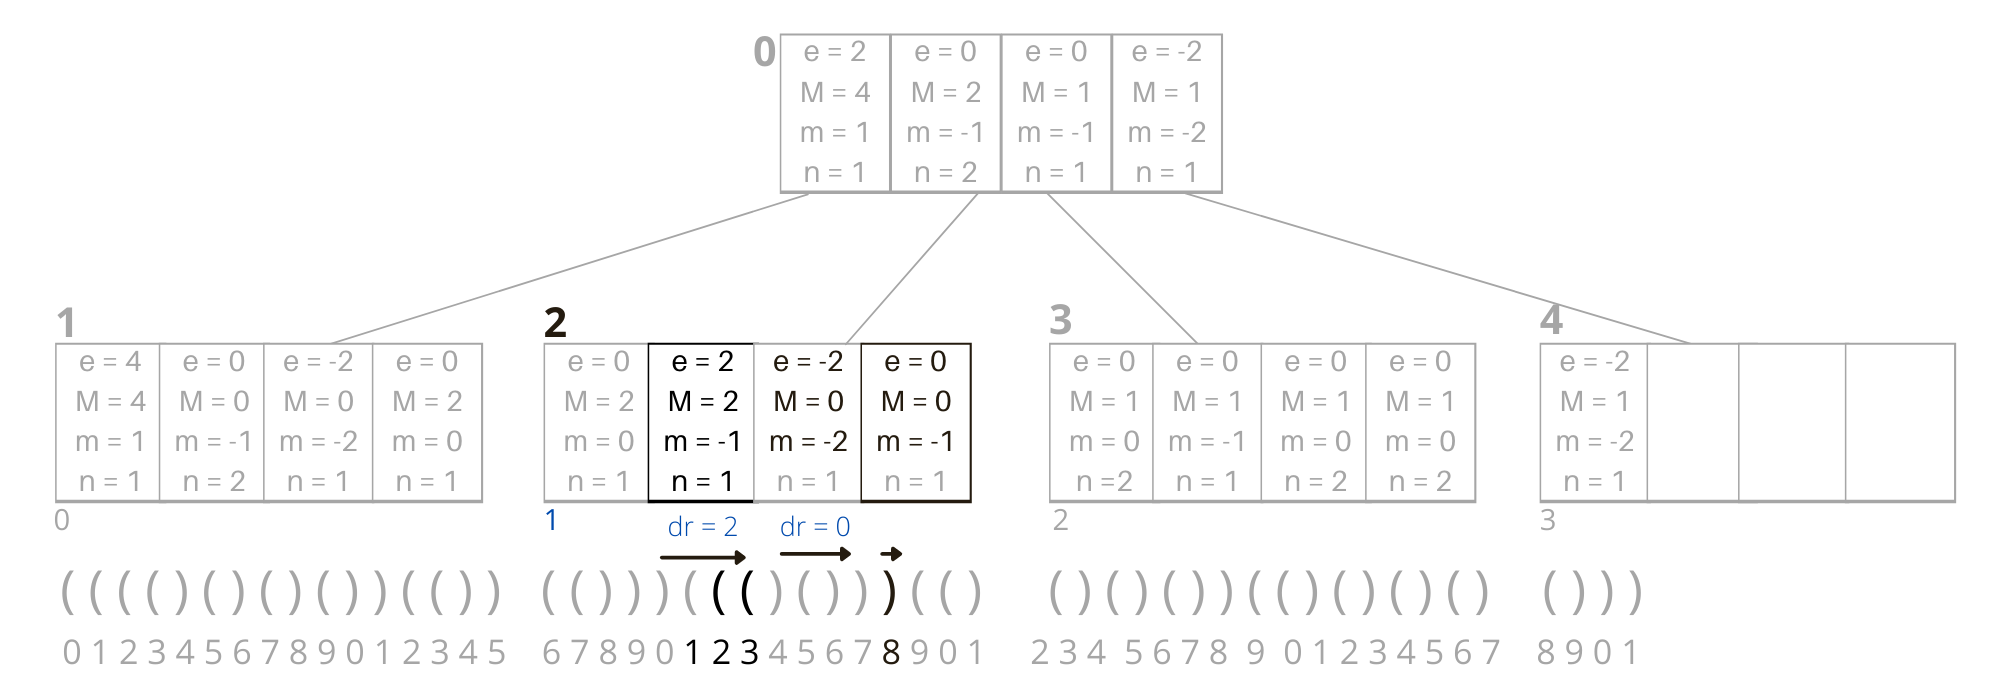
\includegraphics[width=\columnwidth]{images/rmm-tree-kary-fwdsearch.png}
              \label{fig:kary-fwdSearch}
         \end{figure}
        \end{example}
         

\subsection{BwdSearch}\label{sec:bwdSearch}
Como dito anteriormente, o processo para calcular bwdSearch é completamente análogo à fwdSearch, devendo termos cuidado apenas com as questões relacionadas a
simetria dos dados abordadas no capítulo~\ref{ch:fundamentacao}. Tendo isso em mente podemos construir uma função que verifica se o excesso buscado está entre as chaves das
folhas analisadas, assim como uma segunda função para inspecionarmos as chaves dos $p$ vizinhos de um nó $v$ visitado durante o processo de subida e descida na árvore.
Os algoritmos \ref{alg:bwdKey}, \ref{alg:bwdVerifySibling} e \ref{alg:bwdSearch} mostram o pseudocódigo para as adaptações da estrutura multi-ária.

%TODO colocar referência interna
Apenas para reafirmar, temos as seguintes observações em relação à assimetria dos dados em relação a bwdSearch\footnote{Para mais detalhes, verificar seção~\ref{sc:bwdsearch}}:
\begin{itemize}
    \item A posição $i$ é incluída na contagem de excessos;
    \item Adicionamos $1$ à $dr$ quando passamos por um bit $0$, e subtraímos $1$ de $dr$ quando passamos por um bit $1$;
    \item $excess(i) + d $ é alcançado quando $dr - R[v].e + R[v].m \leq d \leq dr - R[v].e + R[v].M $ for verdadeiro.
\end{itemize}

\begin{algorithm}[h!]
    \Input{Nó $v$ e folha correspondente $k$, posição a partir do qual devemos iniciar a busca (índice $i$ e $key$),  excesso relativo buscado e excesso relativo computado em cada chave inspecionada ($d$ e $\&dr$). }
    \Output{Posição $j$ ou $-1$ caso $d$ não seja encontrado.}
    \vspace{.3cm}
    \For{$key$ \textbf{downto}  $0$}{
        \If{$(dr - R[v].keys[key].e + R[v].keys[key].m \leq d \leq dr - R[v].keys[key].e + R[v].keys[key].M)$}{
            $j \leftarrow bwdBlock(i,d,\&dr)$\tcp{Análogo ao algoritmo~\ref{alg:fwdBlock}}
            \lIf{$dr = d$}{ \Return{$j$}}

        }
        $dr \leftarrow dr -  R[v].keys[key].e$\\ 
        $i \leftarrow (m*k+key)*b-1$ \tcp{calcula o início da chave atual}
        \lIf{$dr = d$}{\Return{$i$ }}
    }
    \Return{$-1$ }
\caption{Verificando as chaves de um nó folha através de  $bwdKey(i,v,key,k,d,\&dr)$}
\label{alg:bwdKey}
\end{algorithm}

\begin{algorithm}[h!]
    \Input{Nó $\&v$,  excesso relativo buscado e excesso relativo computado em cada chave inspecionada ($d$ e $\&dr$). }
    \Output{$key$ ou $-1$ caso o intervalo que contém $d$ não seja encontrado.}
    \vspace{.3cm}
    $parent \leftarrow \floor{(v-1)/m}$ \\
    $n\_sibling \leftarrow v - (parent * m) -1 $\\
    $v \leftarrow v - 1$\\
    \While{$n\_sibling$ \textbf{downto}  $0$ \textbf{and} $v$ \textbf{downto} $0$}{
        \For{$key \leftarrow R[v].nKeys -1$ \textbf{to} $0$}{
            \If{$(dr - R[v].keys[key].e + R[v].keys[key].m \leq d)$ \textbf{and} $(d \leq dr - R[v].keys[key].e + R[v].keys[key].M)$}{
                \lIf{$v \leq numberNodes - numberLeaves$}{$v \leftarrow (v*m)+1+key$}
                \Return{$key$ }
            }
            $dr \leftarrow dr -  R[v].keys[key].e$\\
            \lIf{$dr = d$}{
                \lIf{$v \leq numberNodes - numberLeaves$}{$v \leftarrow (v*m)+key$}
                \Return{$key$ }
            }
        }
        \lIf{$n\_sibling -1 > 0$}{$v \leftarrow v-1$}
        $n\_sibling \leftarrow n\_sibling - 1$\\
    }
    \Return{$-1$}
    \caption{Busca o excesso relativo nos irmãos de $v$ através de $bwdVerifySibling(\&v,\&dr,d)$}
    \label{alg:bwdVerifySibling}
\end{algorithm}

\begin{algorithm}[h!]
    \Input{Índice $i$ a partir do qual a busca deve ser feita e excesso relativo buscado $d$. }
    \Output{Posição $j$ onde ocorre o excesso $d$ ou $-1$ caso $d$ não exista no intervalo definido.}
    \vspace{.3cm}
        $dr \leftarrow 0$\\
        $k \leftarrow \floor{i/(b*m)}$\\
        $v \leftarrow leafInTree(k)$\\
        $key \leftarrow \floor{((i+1) - (k*b*m))/b}$\\
        $j \leftarrow bwdBlock(i,d,\&dr)$\tcp{Análogo ao algoritmo~\ref{alg:fwdBlock}}
        \lIf{$dr = d $}{\Return{$j$}}

        $key \leftarrow key -1$\\
        \If{$key \geq 0$}{
            $j \leftarrow bwdKey((m*k+key+1)*b-1,v,key,k,d,\&dr)$\\
            \lIf{$dr = d $}{\Return{$j$}}

        }
        \vspace{.3cm}
        \tcp{Inicia o processo de subida na rmM-tree}
        \While{$v \neq 0$ \textbf{and} $bwdVerifySibling(\&v,\&dr,d) = -1$ }{
            $v \leftarrow \floor{(v-1)/m}$\\
        }
        \tcp{Chegamos ao nó raíz,  mas $d$ não está em nenhum dos seus filhos}
        \If{$v=0$ \textbf{and} $key=-1$}{\Return{$-1$}}
        \vspace{.3cm}
        \tcp{Desce nível a nível da árvore, até que $v$ corresponda ao índice de um dos nós folhas}
        \While{$v \leq numberNodes - numberLeaves$}{
            \For{$key \leftarrow R[v].nKeys - 1$ \textbf{to} $0$}{
                \If{$(dr - R[v].keys[key].e +R[v].keys[key].m \leq d \leq dr - R[v].keys[key].e +R[v].keys[key].M)$}{
                    $v \leftarrow (v*m) + 1 + chave $\\
                    $key \leftarrow R[v].nKeys-1 $\\
                    \textbf{break}
                }
                \lElse{
                    $dr \leftarrow dr - R[v].keys[key].e$
                }

            }
        }
        \vspace{.3cm}
        $k \leftarrow numLeaf(v)$\\
        \lIf{$d = dr$}{\Return{$(k*m*b) + (key*b)-1$}}
        $j \leftarrow bwdKey((k*m*b)+((key+1)*b)-1, v,key,k,d,\&dr)$
        \lIf{$dr = d$}{ \Return{$j$}}
        \lElse{
            \Return{$-1$}
        }
    \caption{Busca por excesso no intervalo $[i+1,BP.size()-1]$ através de $bwdSearch(i,d)$}
    \label{alg:bwdSearch}
    \end{algorithm}

    \begin{example}
    Dado um nó em $BP$, codificado em $i=50$, encontrar o  índice $j<i$ mais à direita de $i$,tal que $excess(j) - excess(i) = 0$.
    \begin{figure}[!ht]
        \centering
          \caption[bwdSearch(50,0).]{Simulação da operação \textit{bwdSearch(50,0)}.}
          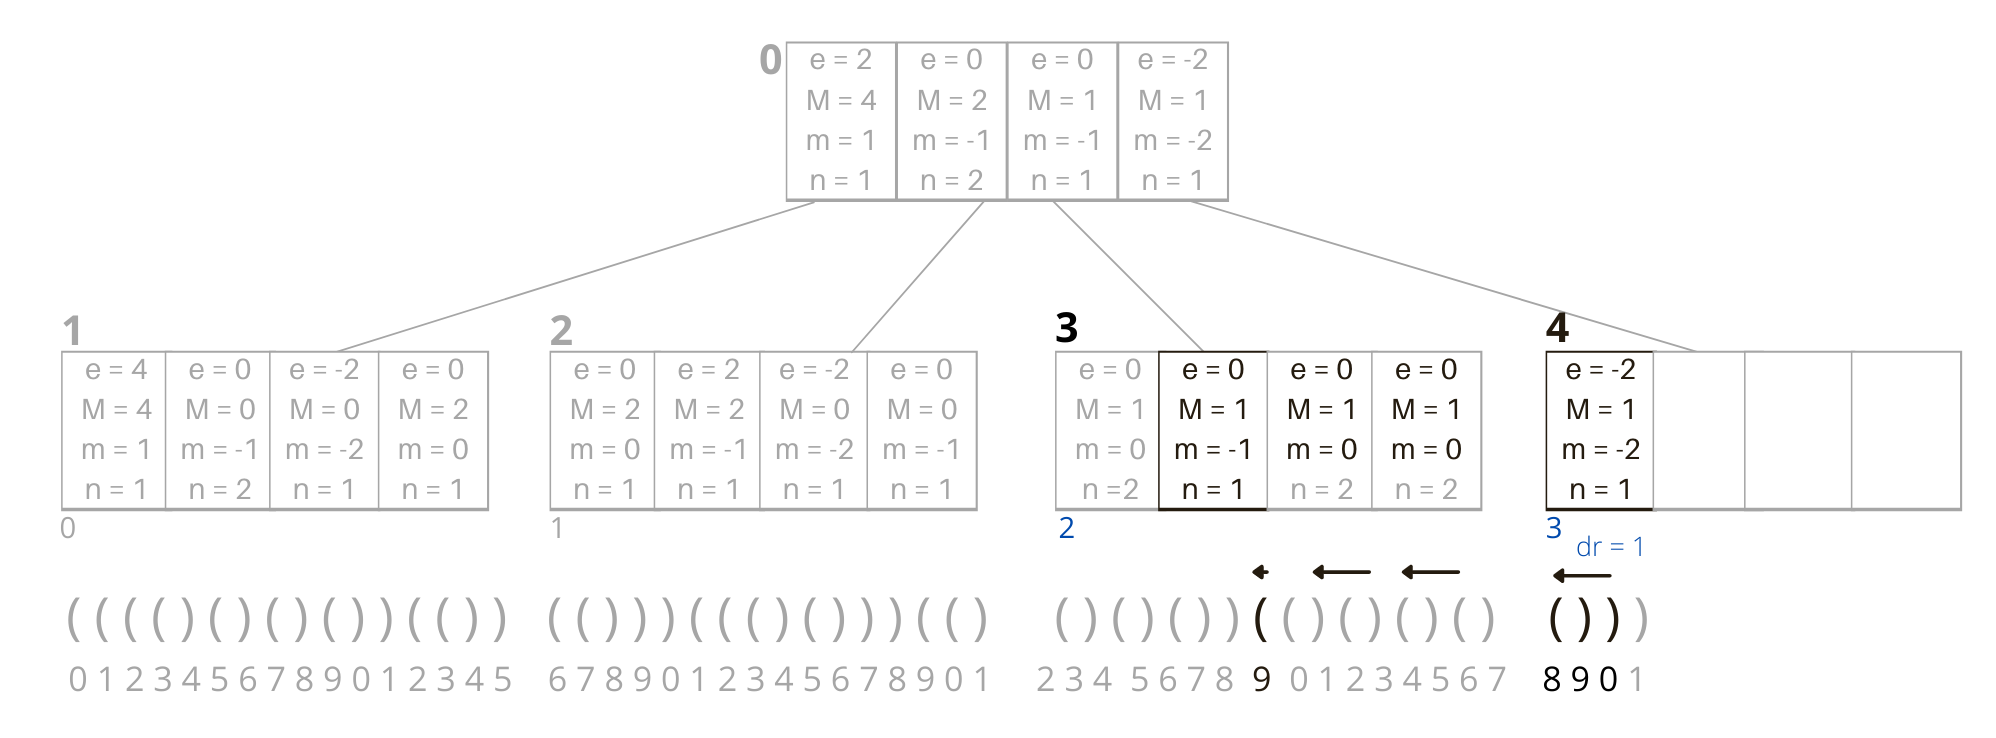
\includegraphics[width=\columnwidth]{images/rmm-tree-kary-bwdsearch.png}
          \label{fig:kary-bwdSearch}
     \end{figure}


     Ao identificarmos o nó a qual pertence o índice $i=50$, temos que $v=4$, temos também que a chave onde se localiza esse índice é a primeira deste nó, 
     ou seja $0$ ($\floor{(50-48)/4}$). 
     
     Inspecionamos a chave deste nó partindo de $i=50$, até chegar ao início da mesma que é $s=48$, ao terminarmos esta inspeção temos que $dr=1$, como ternminarmos
     de inspecionar as chaves deste nó, verificamos quantos irmãos $v$ possuí a sua esquerda, afim de inspecionarmos os mesmos. 
     Atualizamos $v$ para o seu antecessor, que passa a valer $3$, pecorremos então cada chave de $v$ 
     buscando a chave onde a asserção $(dr - R[3].keys[l].e + R[3]].keys[l].m \leq d \leq dr - R[3].keys[l].e + R[3].keys[l].M)$
     é válida. Ao  verificarmos a chave de número $3$ do nó $3$, percebemos que a asserção definida não é válida, seguimos para a chave que precede a atual ($2$), 
     e temos que $d$ não está incluso nos intervalos de excesso mínimo e máximo da chave $2$,
     atualizamos então a chave corrente para $1$, e a asserção é validada. Como encontramos a chave que contém $d$, interrompemos a verificação dos nós da rmM-tree,
    e iniciamos uma varredura bit a bit, do intervalo desta chave.
     Ao realizarmos a inspeção da chave $1$, do nó $3$, encontramos $dr=d$ em $j=49$.
     

     Para este exemplo fizemos a inspeção dos campos de $3$ nós (excluindo o nó inicial), não sendo necessário subir na rmM-tree, já para a estrutura binária, 
     como visto anteriormente, foi necessário, realizar a inspeção de 
     $6$ nós (excluindo o nó inicial), subindo $1$ nível da estrutura, e depois descendo $2$ níveis.
     
    \end{example}

     \subsection{Derivadas}
     Não entraremos nos detalhes das operações derivadas de \textit{fwdSearch} e \textit{bwdSearch}, tendo em vista que as mesmas já foram abordadas anteriormente. 
     Ademais, a tabela~\ref{tbl:karyOperations-rmm-tree} lista as operações suportadas pela nossa implementação da rmM-tree k-ária até o momento de escrita deste trabalho, 
    observe que ela não traz operações como a de menor ancestral comum ($lca$), e obtenção de filho mais profundo de um nó ($deepestNode$), 
     isso ocorre porque as operações que são bases para estas ainda não foram implementadas, entretanto, destaca-se que o processo de adaptação destas operações base é muito similar ao que já foi exposto até aqui.

     \begin{table}[h!]
	\centering
	\caption[Operações sobre a rmM-tree binária e k-ária]{Operações suportadas pela rmM-tree binária e rmM-tree-kária}
	\label{tbl:karyOperations-rmm-tree}
	\rowcolors{2}{lightgray!30}{white}
	\resizebox{\columnwidth}{!}{
	\begin{tabular}{lll}
	\toprule
	\textbf{Operação} & \textbf{rmM-tree binária} & \textbf{rmM-tree k-ária}\\
	\toprule
    
	fwdSearch(i,d)  &  \cmark \par &   \cmark \par\\
	bwdSearch(i,d)  &  \cmark \par &   \cmark \par\\
	minExcess(i,j) / maxExcess(i,j)  &   \cmark \par & \xmark \\
	minCount(i,j)  &   \cmark \par & \xmark\\
	minSelectExcess(i,j,t)  &  \cmark \par & \xmark\\
	enclose(i) &  \cmark \par &   \cmark \par \\
	rmq(i,j) / rMq(i,j) &  \cmark \par & \xmark \\
	rank$_1$(i) / rank$_0$(i) &  \cmark \par &    \cmark \par\\
    select$_1$(i) / select$_0$(i) &  \cmark \par &   \cmark \par\\
    preRank(i)/postRank(i) &  \cmark \par &   \cmark \par\\
    preSelect(i)/postSelect(i) &  \cmark \par &   \cmark \par \\
    isLeaf(i) &  \cmark \par &   \cmark \par\\
    isAncestor(i,j) &  \cmark \par &   \cmark \par\\
    depth(i) &   \cmark \par &   \cmark \par\\
    parent(i) &  \cmark \par &   \cmark \par\\
    firstChild(i) / lastChild(i) &  \cmark \par &   \cmark \par\\
    child(i,t)&  \cmark \par & \xmark \\
    nextSibling(i) / prevSibling(i) &   \cmark \par &   \cmark \par\\
    subtreeSize(i) &   \cmark \par &   \cmark \par\\
    levelAncestor(i,d) &   \cmark \par &   \cmark \par \\
    levelNext(i) / levelPrev(i) &   \cmark \par &   \cmark \par \\
    levelLeftMost(d) / levelRightMost(d) &  \cmark \par &   \cmark \par\\
    lca(i,j)&  \cmark \par & \xmark\\
    deepestNode(i)&  \cmark \par & \xmark \\
    degree(i)&  \cmark \par & \xmark\\
    childRank(i)&  \cmark \par & \xmark\\
    leafRank(i)&  \cmark \par &   \cmark \par\\
    leafSelect(i)&  \cmark \par  &   \cmark \par\\
    leftMostLeaf(i)&   \cmark \par &   \cmark \par\\
    rightMostLeaf(i)&   \cmark \par &   \cmark \par\\
	\bottomrule
	\end{tabular}
	}
\end{table}




%base de dados, configuração, experimentos, resultados
%figura, resultado destacado.